\exercise{1} \points{14}\\
Implement a class \emph{BinarySearchTree} with a binary search tree, such that 
the keys are of type \emph{int} (integer) and the elements of type \emph{str} (string).

Please note that only \emph{insert} (6 points) and \emph{lookup} (4 points), 
but not \emph{remove} needs to be implemented. This means that you can omit the 
doubly linked lists between the nodes in your tree.

\begin{figure}[b]
  \begin{center}
    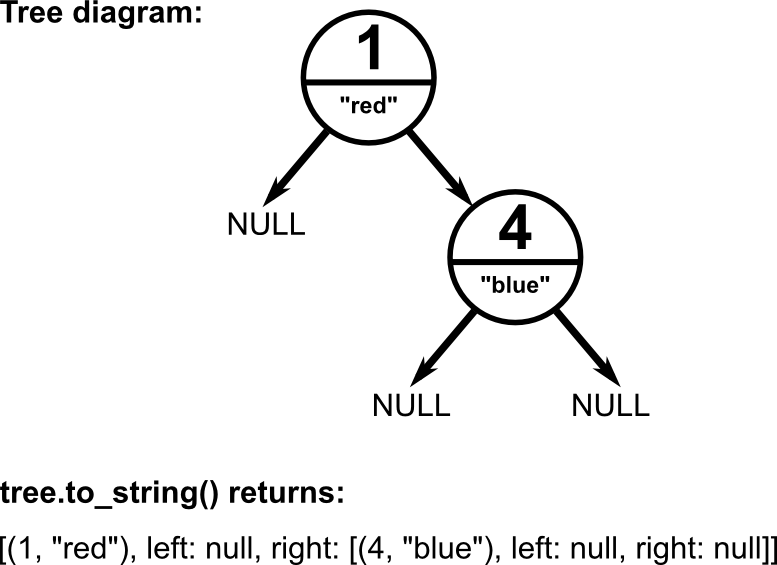
\includegraphics[width=0.6\textwidth]{Images/diagram.png}
  \end{center}
\caption{example tree diagram and corresponding output string of the to\_string method.}
\label{fig:diagram}
\end{figure}

As usual, write some (useful) tests for your methods. For this purpose write 
one \emph{to\_string} method (4 points) which outputs a string representation of your binary tree (see Figure~\ref{fig:diagram} for illustration).
